\chapter{Image Processing}
\label{cha:IP}

\begin{table}[h]\small
    \begin{tabular}{c|ccc}
    \hline 
    Colour&Red Value&Green Value&Blue Value\\
    \hline 
    Green(A1)&67&180&131\\
    Red(A2)&226&90&77\\
    Orange(B1)&255&189&124\\
    Blue(B2)&48&158&228\\
    \hline 
    \end{tabular}
    \end{table}

\subsection{Known Issues}

\begin{enumerate}
    \item[1)] The theta of self robot is calculated wrongly some times, since the rear of self robot is not recognized.
    \item[2)] Once any part of robot move out of the map (as shown in Figure \ref{wrong_position}), the code will report an error that the access error as shown in Figure \ref{access_error}. This is the reason that the algorithm is trying to read a memory address is out of the map, which is larger than the coordinates of image. But according to the competition rules, this should be avoided.
\end{enumerate}

\begin{figure}[thb]
    \centering
    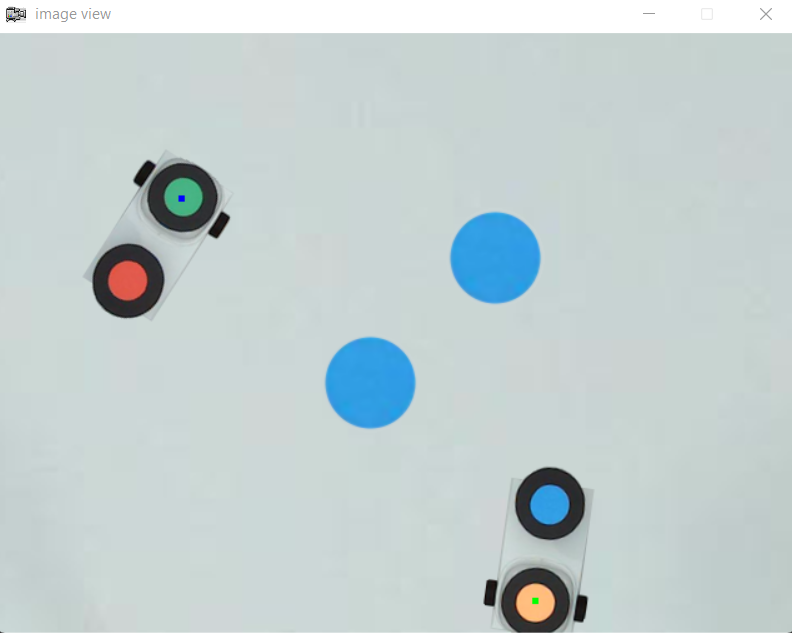
\includegraphics[width=1\textwidth]{images/wrong_position.png}
    \caption[wrong position]{an example of positions that will cause the problem.}\label{wrong_position}
\end{figure}

\begin{figure}[thb]
    \centering
    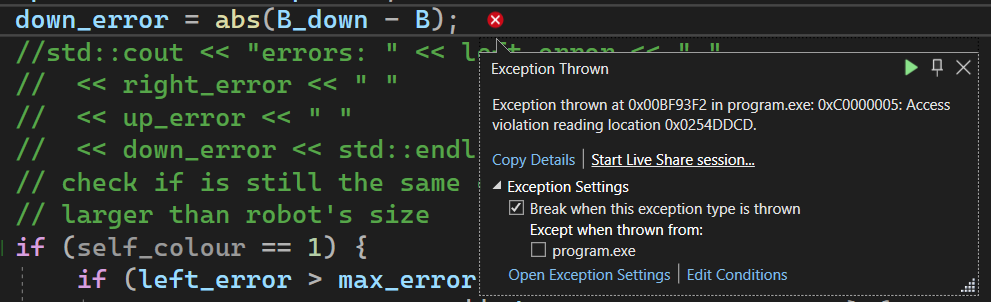
\includegraphics[width=1\textwidth]{images/access_error.png}
    \caption[access error]{access error that happens while at the wrong positions.}\label{access_error}
\end{figure}

